% !TeX root = RJwrapper.tex 
\title{A Computational Analysis of the Dynamics of R Style Based on 108 Million Lines of Code from All CRAN Packages in the Past 21 Years}
\author{by Chia-Yi Yen, Mia Huai-Wen Chang, Chung-hong Chan}

\maketitle

\abstract{
The flexibility of R and the diversity of the R community leads to a large number of programming styles applied in R packages. We have analyzed 108 million lines of R code from CRAN and quantified the evolution in popularity of 12 style-elements from 1998 to 2019. We attribute 3 main factors that drive changes in programming style: effect of style-guides, effect of introducing new features, and effect of editors. A consensus in programming style is forming and we have summarized it into a style which contains all of the most popular style elements, e.g. snake case, use <- for assignment etc.
\footnote{
    We have presented a previous version of this paper as a poster at UseR! 2019 Toulouse. Interested readers can access it with the following link: \url{
    https://github.com/chainsawriot/rstyle/blob/master/Poster_useR2019_Toulouse.png}
}
}

\section{Introduction}

R is flexible. For example, one can use \code{<-} or \code{=} as assignment operators. The following two functions can both be correctly evaluated.

\begin{example}
sum_of_square <- function(x) {
    return(sum(x^2))
}
\end{example}

\begin{example}
sum_oF.square=function(x)
{
    sum(x ^ 2)}
\end{example}

One area that can highlight this flexibility is naming conventions. According to the previous research by \citet{baaaath}, there are at least 6 styles and none of the 6 has dominated the scene. Beyond naming conventions investigated by Baath, there are style-elements that R programmers have the freedom to adopt, e.g. whether or not to add spaces around infix operators, use double quotation marks or single quotation marks to denote strings, etc. On one hand, these variations provide programmers with freedom. On the other hand, these variations can confuse new programmers and can have dire effects on program comprehension. Also, incompatibility between programming styles might also affect reusability, maintainability \citep{elish}, and open source collaboration \citep{wang}. 

Various efforts to standardize the programming style, e.g. Google's R Style Guide \citep{google}, the Tidyverse Style Guide \citep{tidyverse}, Bioconductor Coding Style \citep{bioconductor} etc.,  are available (Table~\ref{tab:table1}) \footnote{\citet{baaaath} lists also \href{https://csgillespie.wordpress.com/2010/11/23/r-style-guide/}{Colin Gillespie's R style guide}.  Additional style guides that we found include the style guides by \href{https://docs.google.com/document/d/1esDVxyWvH8AsX-VJa-8oqWaHLs4stGlIbk8kLc5VlII/edit}{Henrik Bengtsson}, \href{https://jef.works/R-style-guide/}{Jean Fan}, \href{https://irudnyts.github.io//r-coding-style-guide/}{Iegor Rudnytskyi}, \href{https://rpahl.github.io/r-some-blog/my-r-style-guide/}{Roman Pahl}, \href{https://cran.r-project.org/web/packages/rockchalk/vignettes/Rstyle.pdf}{Paul E. Johnson}, \href{https://bookdown.org/joshuah40/qa_code/Coding-Guidelines.html}{Joshua Halls},  \href{https://www.datanovia.com/en/blog/r-coding-style-best-practices/}{Datanovia}, and \href{https://www.daqana.org/dqstyle-r/}{daqana}. We focus only on the 3 style guides of Tidyverse, Google and Bioconductor is because these 3 are argubly the most influential. There are groups of developers (e.g. contributers to \CRANpkg{tidyverse}, Google employees, and Bioconductor contributors) adhering to these 3 styles.}.

Among the 3 style-guides, the major differences are the suggested naming convention and indentation. Other style-elements are essentially the same. These style guides are based on possible improvement in code quality, e.g. style-elements that improve program comprehension \citep{oman}. However, we argue that one should first study the current situation, and preferably, the historical development, of programming style variations (PSV) to supplement these standardization efforts. We have undertaken such a task, so that the larger R communities can have a baseline to evaluate the effectiveness of those standardization efforts. Also, we can have a better understanding of the factors driving increase and decrease in PSV historically, such that more effective standardization efforts can be formulated.

\newcolumntype{L}{>{\centering\arraybackslash}m{3cm}}

\begin{table}

\caption{\label{tab:table1}Three major style-guides: Google, Tidyverse and Bioconductor}
\centering
\begin{tabular}[t]{L|L|L|L}
\hline
Feature & Google & Tidyverse & Bioconductor\\
\hline
\textbf{Function name} & UpperCamel & snake\_case & lowerCamel\\
\hline
Assignment & Discourage = & Discourage = & Discourage =\\
\hline
Line length & “limit your code to 80 characters per line” & “limit your code to 80 characters per line” & $\leqslant$ 80\\
\hline
Space after a comma & Yes & Yes & Yes\\
\hline
Space around infix operators & Yes & Yes & Yes\\
\hline
\textbf{Indentation} & 2 spaces & 2 spaces & 4 spaces\\
\hline
Integer & Not specified & Not specified (Integers are not explicitly typed in included code examples) & Not specified\\
\hline
Quotes & Double & Double & Not specified\\
\hline
Boolean values & Use TRUE / FALSE & Use TRUE / FALSE & Not specified\\
\hline
Terminate a line with a semicolon & No & No & Not specified\\
\hline
Curly braces & \{ same line, then a newline, \} on its own line & \{ same line, then a newline, \} on its own line & Not specified\\
\hline
\end{tabular}
\end{table}


\section{Analysis}
\subsection{Data Source}

On July 1, 2020, we cloned a local mirror of CRAN using the rsync method suggested in the CRAN Mirror HOWTO \citep{cranminihowto}. Our local mirror contains all packages as tarball files (.tar.gz). By all packages, we mean packages actively listed online on the CRAN website as well as orphaned and archived packages. In this analysis, we include all active, orphaned and archived packages.

In order to facilitate the analysis, we have developed the package \code{baaugwo} \citep{chan2} to extract all R source code and metadata from these tarballs. In this study, only the source code from the \code{/R} directory of each tarball file is included. We have also archived the metadata from the \code{DESCRIPTION} and \code{NAMESPACE} files from the tarballs.

In order to cancel out the over-representation effect of multiple submissions in a year by a particular package, we have applied the \emph{"one-submission-per-year"} rule to randomly selected only one submission from a year for each package. Unless explicitly notice, we present below the analysis of this \emph{"one-submission-per-year"} sample. Similarly, unless explicitly notice, the unit of the analysis is \emph{exported function}. The study period for this study is from 1998 to 2019.

\subsection{Quantification of PSV}

Every exported function in our sample are parsed into a parse tree using the parser from the \CRANpkg{lintr} \citep{lintr} package.

These parse trees were then filtered for lines with function definition and then linted them using the linters from the lintr package to detect for various style-elements. Style-elements considered in this study are:

\paragraph{fx\_assign}

Use = as assignment operators

\begin{example}
softplusFunc = function(value, leaky = FALSE) {
    if (leaky) {
        warnings("using leaky RELU!")
        return(ifelse(value > 0L, value, value * 0.01))
    }
    return(log(1L + exp(value)))
}
\end{example}

\paragraph{fx\_opencurly}

An open curly is on its own line

\begin{example}
softplusFunc <- function(value, leaky = FALSE) 
{
    if (leaky) 
    {
        warnings("using leaky RELU!")
        return(ifelse(value > 0L, value, value * 0.01))
    }
    return(log(1L + exp(value)))
}
\end{example}

\paragraph{fx\_infix}

No spaces are added around infix operators.

\begin{example}
softplusFunc<-function(value, leaky=FALSE) {
    if (leaky) {
        warnings("using leaky RELU!")
        return(ifelse(value>0L, value, value*0.01))
    }
    return(log(1L+exp(value)))
}
\end{example}

\paragraph{fx\_integer}

Not explicitly type integers

\begin{example}
softplusFunc <- function(value, leaky = FALSE) {
    if (leaky) {
        warnings("using leaky RELU!")
        return(ifelse(value > 0, value, value * 0.01))
    }
    return(log(1 + exp(value)))
}
\end{example}

\paragraph{fx\_singleq}

Use single quotation marks for strings

\begin{example}
softplusFunc <- function(value, leaky = FALSE) {
    if (leaky) {
        warnings('using leaky RELU!')
        return(ifelse(value > 0L, value, value * 0.01))
    }
    return(log(1L + exp(value)))
}
\end{example}

\paragraph{fx\_commas}

No space is added after commas

\begin{example}
softplusFunc <- function(value,leaky = FALSE) {
    if (leaky) {
        warnings("using leaky RELU!")
        return(ifelse(value > 0L,value,value * 0.01))
    }
    return(log(1L + exp(value)))
}
\end{example}

\paragraph{fx\_semi}

Use semicolons to terminate lines

\begin{example}
softplusFunc <- function(value, leaky = FALSE) {
    if (leaky) {
        warnings("using leaky RELU!");
        return(ifelse(value > 0L, value, value * 0.01));
    }
    return(log(1L + exp(value)));
}
\end{example}

\paragraph{fx\_t\_f}

Use T/F instead of TRUE / FALSE

\begin{example}
softplusFunc <- function(value, leaky = F) {
    if (leaky) {
        warnings("using leaky RELU!")
        return(ifelse(value > 0L, value, value * 0.01))
    }
    return(log(1L + exp(value)))
}
\end{example}

\paragraph{fx\_closecurly}

An close curly is not on its own line.

\begin{example}
softplusFunc <- function(value, leaky = FALSE) {
    if (leaky) {
        warnings("using leaky RELU!")
        return(ifelse(value > 0L, value, value * 0.01)) }
    return(log(1L + exp(value))) }
\end{example}

\paragraph{fx\_tab}

Use tab to indent

\begin{example}
softplusFunc <- function(value, leaky = FALSE) {
    if (leaky) {
        warnings("using leaky RELU!")
        return(ifelse(value > 0L, value, value * 0.01))
    }
    return(log(1L + exp(value)))
}
\end{example}

We have studied also the naming conventions of all included functions. Using the similar technique of \citet{baaaath}, we classified function names into the following 7 categories:

\begin{itemize}
  \item \textbf{alllower} softplusfunc
  \item \textbf{ALLUPPER} SOFTPLUSFUNC
  \item \textbf{UpperCamel} SoftPlusFunc
  \item \textbf{lowerCamel} softPlusFunc
  \item \textbf{lower\_snake} soft\_plus\_func
  \item \textbf{dotted.func} soft.plus.func
  \item \textbf{other} sOfTPluSfunc
\end{itemize}

The last style-element is line-length. For each R file, we counted the distribution of line-length. In this analysis, the unit of analysis is line.

If not considering line-length, the remaining 10 binary and one multinomial leave 7,168 possible combinations of PSVs that a programmer could employ ($7 \times 2^{10} = 7,168$).

\subsection{Community-specific variations}

On top of the overall patterns based on the analysis of all functions, the community-specific variations are also studied. In this part of the study, we ask the question: do local patterns of PSV exist in various programming communities? To this end, we constructed a dependency graph of CRAN packages by defining a package as a node and an import/suggest relationship as a directed edge. Communities in this dependency graph were extracted using the Walktrap Community Detection Algorithm \citep{pons} provided by the \CRANpkg{igraph} package \citep{csardi}. The step parameter was set at 4 for this analysis. Notably, we analyzed the dependency graph as a snapshot, which is built based on the latest submission of each package in or before 2019.

We selected the largest 20 communities for further analysis. The purpose of this analysis is to show the PSV across communities. The choice of 20 is deemed enough to show these community-specific variations. Readers could explore other choices themselves using our openly shared data.

\section{Results}

We studied more than 94 million lines of code from 15,530 unique packages. In total, 1,898,142 exported functions were studied. Figure~\ref{figure:fig1} displays the popularity of the 10 binary style-elements from 1998 to 2008. Some style-elements have very clear trends towards a majority-vs-minority pattern, e.g. fx\_closecurly, fx\_semi, fx\_t\_f and fx\_tab. Some styles-elements are instead trending towards a divergence from a previous majority-vs-minority pattern, e.g. fx\_assign, fx\_commas, fx\_infix, fx\_integer, fx\_opencurly and fx\_singleq. There are two style-elements that deserve special scrutiny. Firstly, the variation in fx\_assign is a clear example illustrating the effect of introducing a new language element by the R Development Core Team. The introduction of the language feature (= as assignment operator) in R 1.4 \citep{chambers} has coincided with the taking off in popularity of such style-element since 2001. Up to now, around 20\% of exported functions use such style.

\begin{figure}[htbp]
  \centering
  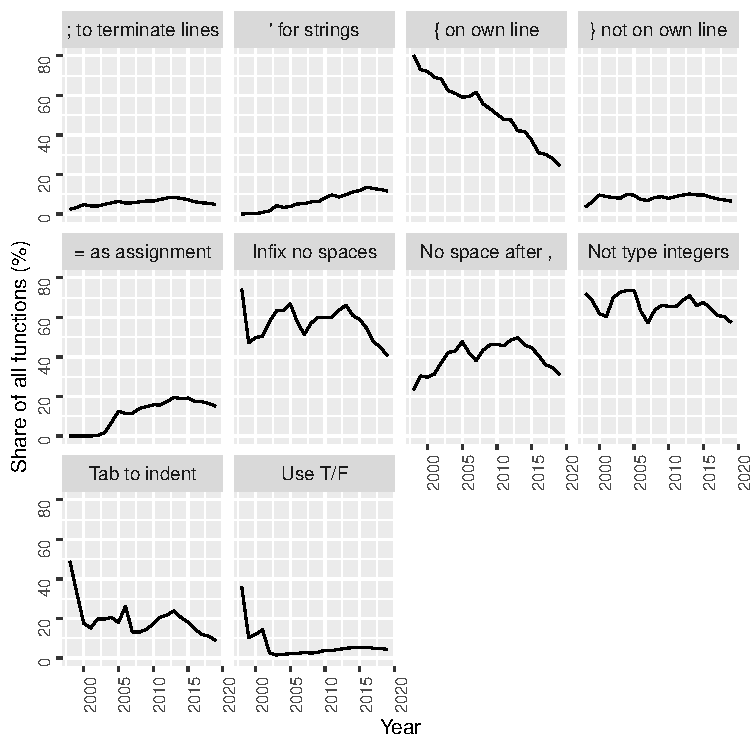
\includegraphics{fig1}
  \caption{Evolution in popularity of 10 style-elements from 1998 to 2019.}
  \label{figure:fig1}
\end{figure}


Secondly, the popularity of fx\_opencurly shows how a previously established majority style (~80\% in late 90s) slowly reduced into a minority but still very prominent style (~30\% in late 10s).

Similarly, the evolution of different naming conventions is shown in Figure~\ref{figure:fig2} \footnote{'Other' is the 4th most popular naming convention. Some examples of function names classified as 'other' are: \emph{Blanc-Sablon}, \emph{returnMessage.maxim}, \emph{table\_articles\_byAuth}, \emph{mktTime.market}, \emph{smoothed\_EM}, \emph{plot.Sncf2D}, \emph{as.igraph.EPOCG}, \emph{TimeMap.new}, \emph{fT.KB}, \emph{IDA\_stable}. These functions were classified as 'other' because of the placement of capital letters. For packages using an all capitals object class name (e.g. EPOCG) and S3 generic method names (e.g. as.igraph), their methods are likely to be classified as 'others'. One could also classify these functions as dotted.func. However, we follow both \CRANpkg{lintr} and \citet{baaaath} to classify a function as dotted.func only when no capital letter is used in its name.}. This analysis can best be used to illustrate the effect of style-guides. According to \citet{baaaath}, dotted.func style is very specific to R programming. This style is the most dominant style in the early days of CRAN. However, multiple style guides advise against the use of dotted.func style and thus a significant declining trend is observed. lower\_snake and UpperCamel are the styles endorsed by the Tidyverse Style Guide and the Google's R Style Guide, respectively. These two styles see an increasing trend since the 2010s, while the growth of lower\_snake is stronger. In 2019, lower\_snake (a style endorsed by Tidyverse) is the most popular style (26.6\%). lowerCamel case, a style endorsed by Bioconductor, is currently the second most popular naming convention (21.3\% in 2019). Only 7.0\% of functions use UpperCamel, the style endorsed by Google.

\begin{figure}[htbp]
  \centering
  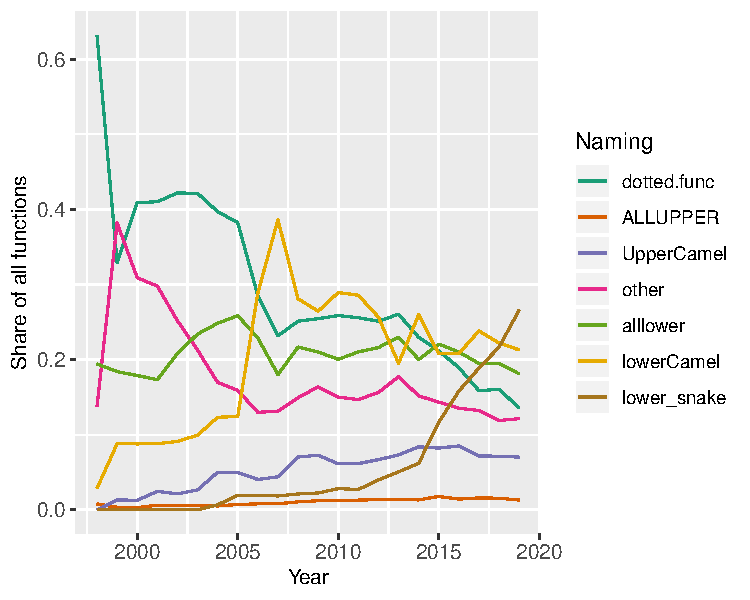
\includegraphics{fig2}
  \caption{Evolution in popularity of 7 naming conventions from 1998 to 2019.}
  \label{figure:fig2}
\end{figure}

The evolution of line lengths is tricky to be visualized on a 2-D surface. We have prepared an animation (\url{https://github.com/chainsawriot/rstyle/blob/master/file60f331694ef5.gif}) to visualize the change in line distribution over the span of 20 years. In this paper, Figure~\ref{figure:fig3} shows the snapshot of the change in line length distribution in the range of 40 to 100 characters. In general, developers of newer packages write with a lesser number of characters per line. Similar to previous analyses with Python programs (e.g. \citet{vanderplas}), artificial peaks corresponding to recommendations from either style-guides, linters, and editor settings are also observed in our analysis. In 2019, the artificial peak of 80 characters (recommended by most of the style-guides and linters such as \CRANpkg{lintr}) is more pronounced for lines with comments but not those with actual code.


\begin{figure}[htbp]
  \centering
  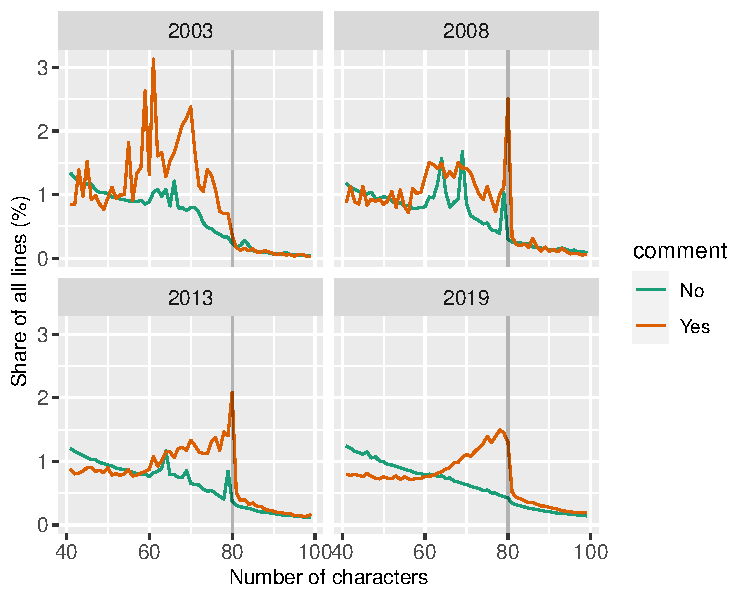
\includegraphics{fig3}
  \caption{Change in line length distribution: 2003, 2008, 2013 and 2019.}
  \label{figure:fig3}
\end{figure}

\subsection{Within-package variations}
Therefore, 11 binary indicators will be assigned to each function within a package, which refers to style variation it adopts. Second, we compute the entropy of these style indicators among all the functions within a package, and therefore we can analyze the consistency of each style element within a package. Notably, we normalize the entropy of style elements to be [0, 1], such that we can compare the entropy across style elements fairly. Finally, we calculate the average entropy of all CRAN packages by aggregating the package-level entropy we computed in the previous stage. 

The result shows that consistency is still an issue for many style elements within a package. For example, style elements like fx\_integer, fx\_commas, fx\_infix, fx\_opencurly, and fx\_name have rather larger variations, compared to fx\_tab, fx\_semi, fx\_t\_f, fx\_closecurly, fx\_singleq, fx\_assign, as shown in the below figure.


This finding echoes our concerns that these inconsistent style variations at package level may hinder developers collaborating in a more efficient way.  We provide a more detailed example in the naming convention (fx\_name) for a better understanding of the within-package style inconsistency, as shown in the below figure.


We list the most important packages identified by their pagerank in the CRAN dependency graph.  As what we expect, lower\_snake or lowerCamel is the dominating naming convention in many packages. However, for many packages like digest, Rcpp, and survival, there is a lack of consensus on the function names, which may make it harder for developers to read the codes in a more efficient way.

\subsection{Community-based variations}

Using the aforementioned community detection algorithm of the dependency graph, 20 large communities were extracted. These communities are named by their applications. Table~\ref{tab:table2} lists the details of these communities.

Using the naming convention as an example, there are local patterns in PSV (Figure~\ref{figure:fig4}). For example, lower\_snake case is the most popular naming convention in the "RStudio-related" community as expected because it is the naming convention endorsed by the Tidyverse Style-guide. However, none of the functions exported by the packages from "Time, Date, and Money" community uses such convention.

\begin{table}

\caption{\label{tab:table2}The largest 20 communities and their top 3 packages according to eigenvector centrality}
\centering
\begin{tabular}[t]{l|r|l}
\hline
Community & Number of Packages & Top 3 Packages\\
\hline
RStudio-related & 3426 & knitr, testthat, rmarkdown\\
\hline
base & 2618 & methods, graphics, lattice\\
\hline
Image Plotting & 2228 & png, rgl, highr\\
\hline
RCpp & 677 & Rcpp, inline, pkgKitten\\
\hline
GPS and Geography & 530 & deldir, sp, maptools\\
\hline
Machine learning & 319 & rpart, nnet, randomForest\\
\hline
Text Analysis & 92 & stopwords, NISTunits, ISOcodes\\
\hline
Social Network Analysis & 53 & texreg, network, ergm\\
\hline
Graphics & 49 & apt, BioIDMapper, Blaunet\\
\hline
Graph data structure & 48 & graph, scagnostics, RBGL\\
\hline
Genetics & 44 & AhoCorasickTrie, BinQuasi, biofiles\\
\hline
Finance & 36 & RUnit, RcppCCTZ, CFL\\
\hline
Insurance and Actuary & 34 & rsp, babar, BALD\\
\hline
Numerical Optimization & 30 & pbivnorm, rgenoud, Matching\\
\hline
Sparse Matrix & 30 & registry, slam, Rsymphony\\
\hline
Java & 28 & rJava, RWekajars, AWR\\
\hline
Neuroscience & 27 & STAR, rstream, extremefit\\
\hline
Time, Date, and Money & 27 & tis, setRNG, CDNmoney\\
\hline
\end{tabular}
\end{table}

\begin{figure}[htbp]
  \centering
  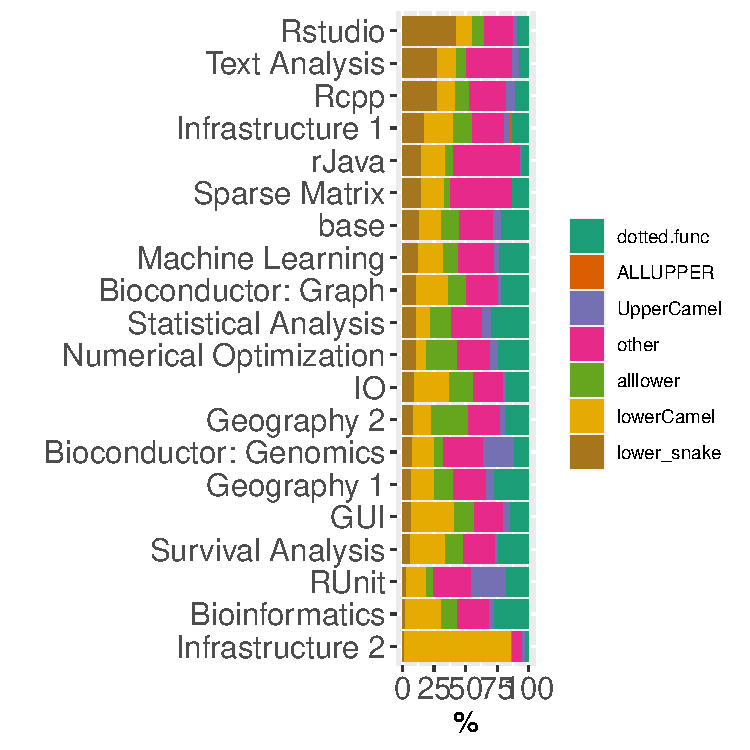
\includegraphics{fig4}
  \caption{Community-specific distribution of naming conventions among 18 large communities.}
  \label{figure:fig4}
\end{figure}

For the binary style-elements, local patterns are also observed (Figure~\ref{figure:fig5}). The most salient pattern is the "Java" and "Sparse Matrix" communities exceptional high usage of tab indentation, probably due to influences from Java or Matlab. Also, the high level in usage of open curly on its own line for the "Graphics" is also exceptional.

\begin{figure}[htbp]
  \centering
  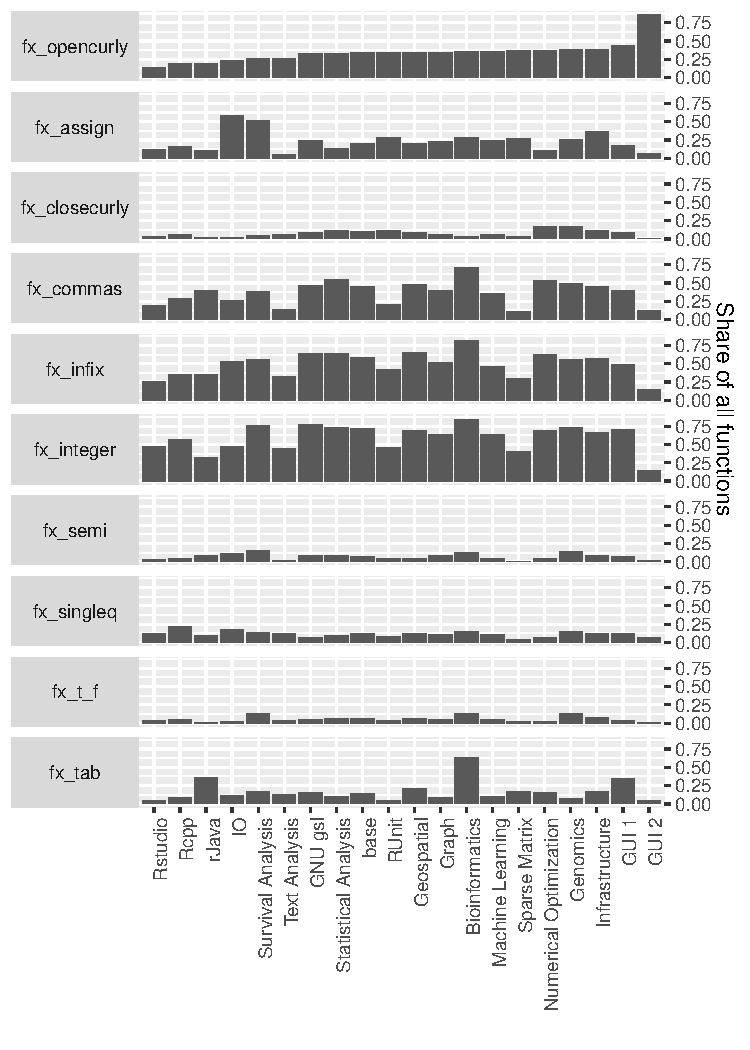
\includegraphics{fig5}
  \caption{Community-specific distribution of style-elements among 18 large communities}
  \label{figure:fig5}
\end{figure}

\section{Discussion}

In this study, we study the PSV in 21 years of CRAN packages across two dimensions: 1) temporal dimension: the longitudinal changes in popularity of various style-elements over 21 years, and 2) cross-sectional dimension: the variations among communities of the latest snapshot of all packages. From our analysis, we identify three factors that possibly drive PSV: effect of style-guides (trending of naming conventions endorsed by \citet{tidyverse} and \citet{google}), the effect of introducing a new language feature (trending of = usage as assignments after 2001), and effect of editors and linters (the dominance of 80-character line limit).

From a policy recommendation standpoint, our study provides important insight for the R Development Core Team and other stakeholders. Firstly, the introduction of a new language can have a very long-lasting effect on PSV. "Assignments with the = operator" is a feature that introduced by the R Development Core Team to ``increase compatibility with S-Plus (as well as with C, Java, and many other languages)'' \citep{chambers}. This might be in a good intention but it has an unintended consequence of introducing a very persistent PSV that two major style-guides, \citet{tidyverse} and \citet{google}, consider as a bad style.

Secondly, style-guides, linters, and editors are important standardizers of PSV. Although we have not directly measured the use of style-guides, linters, and editors in our analysis \footnote{The usage of style-guides, linters, and editors cannot be directly measured from the record on CRAN. The maintainers usually do not explicitly state the style-guide they endorsed in their code. Similarly, packages that have been processed with linters do not import or suggest linters such as \CRANpkg{lintr}, \CRANpkg{styler} or \CRANpkg{goodpractice}. It might be possible to infer the use of a specific editor such as RStudio in the development version of a package with signals such as the inclusion of an RStudio Project file. These signals, however, were usually removed in the CRAN submission of the package. Future research should use alternative methods to measure the usage of these 3 things in R packages.}, we infer their effect by study the time trend (Figure~\ref{figure:fig1}). Even with these standizers, programming styles are slow to change. As indicated by the local patterns of PSV we found in some communities, some package developers keep using their own styles. Having said so, we are not accusing those developers of not following the trendy programming styles. Instead, they follow the mantra of ``if it ain't broke don't fix it''. Again, from a policy recommendation standpoint, the existence of local PSV patterns suggests there are many blind spots to the previous efforts in addressing PSV. Style-guide's authors may consider community outreach to promote their endorsed styles, if they want other communities to adopt their styles.

Our analysis also opens up an open question: should R adopt an official style-guide akin the PEP-8 of the Python Software Foundation \citep{vanrossum}? There are of course pros and cons of adopting an official style-guide. As written by \citet{christiansen}, ``style can easily become a religious issue.'' It is not our intention to meddle in this ``religious issue.'' If such an effort would be undertaken by someone else, we suggest the following consensus-based style. The following is an example of a function written in such style.

\begin{example}
softplus_func <- function(value, leaky = FALSE) {
    if (leaky) {
        warnings("using leaky RELU!")
        return(ifelse(value > 0, value, value * 0.01))
    }
    return(log(1 + exp(value)))
}
\end{example}

In essense,

\begin{itemize}
  \item Use snake case
  \item Use <- to assign, don't use =
  \item Add a space after commas
  \item Use TRUE / FALSE, don't use T / F
  \item Put open curly bracket on same line then a newline
  \item Use double quotation mark for strings
  \item Add spaces around infix operators
  \item Don't terminate lines with semicolon
  \item Don’t explicitly type integers (i.e. 1L)
  \item Put close curly bracket on its own line
  \item Don't use tab to indent
\end{itemize}

We must stress here that this \emph{consensus-based} style is only the most popular style based on our analysis, i.e. the \emph{Zeitgeist} (the spirit of the age) \footnote{In 2019, 5.35\% of all functions are using this \emph{Zeitgeist} style. Using electorial system as an analogy, this style is having the plurality (have the highest number of votes) but not the absolute majority (have over 50\% of the votes)}. We have no guarantee that this style can improve clarity or comprehensibility. As a final remark: although enforcing a consistent style can improve open source collaboration \citep{wang}, one must also bear in mind that these rules might need to be adjusted sometimes to cater for programmers with special needs. For example, using spaces instead of tabs for indentation can make code not accessible to visually impaired programmers \citep{mosal}.

\section{Reproducibility}

The data and scripts to reproduce the analysis in this paper are available at \url{https://github.com/chainsawriot/rstyle}.

\bibliography{RJreferences}

\newpage
\address{Chia-Yi Yen\\
  Mannheim Business School, Universit\"at Mannheim\\
  L 5, 6, 68131 Mannheim\\
  Germany\\
  \url{https://orcid.org/0000-0003-1209-7789}\\
  \email{yen.chiayi@gmail.com}}

\address{Mia Huai-Wen Chang\\
  Akelius Residential Property AB\\
  Erkelenzdamm 11-13, 10999 Berlin\\
  Germany\\
  \email{mia5419@gmail.com}}

\address{Chung-hong Chan\\
  Mannheimer Zentrum f\"ur Europ\"aische Sozialforschung, Universit\"at Mannheim\\
  A5, 6,  68159 Mannheim\\
  Germany\\
  \url{https://orcid.org/0000-0002-6232-7530}\\
  \email{chung-hong.chan@mzes.uni-mannheim.de}}

